\documentclass[11pt,a4j,uplatex]{jsarticle}
\usepackage{ascmac}
\usepackage{amsmath,amssymb}
\usepackage[dvipdfmx]{graphicx}
\usepackage{upgreek}%\upGreek
\usepackage{cases}%連立方程式
\usepackage{bm}%ベクトル表記\bm{A}
\usepackage{bigdelim,multirow}


\newsavebox{\circlebox}
\savebox{\circlebox}{\fontencoding{OMS}\selectfont\Large\char13}
\newlength{\circleboxwdht}
\newcommand{\centercircle}[1]{%
  \setlength{\circleboxwdht}{\wd\circlebox}%
  \addtolength{\circleboxwdht}{\dp\circlebox}%
  \raisebox{0.4\dp\circlebox}{%
    \parbox[][\circleboxwdht][c]{\wd\circlebox}{\centering#1}}%
  \llap{\usebox{\circlebox}}%
}	%丸数字(文字)環境。\centercircle{入れたい文字} で丸文字を表示する。


\title{Semiconductor Optics}
\author{13.1.1-3}

\makeatletter%図番号定義
%\renewcommand{\figurename}{Firuge}%図表記をFigure *.*へ
\renewcommand{\thefigure}{\thesection.\arabic{figure}}%図 章番号.図番号
\makeatletter

\begin{document}
\if0
 \maketitle %タイトル

 \thispagestyle{empty}%このページにはページ番号を入れない.
 \clearpage
 \addtocounter{page}{-1}


 \tableofcontents %目次

 \thispagestyle{empty}%このページにはページ番号を入れない
 \clearpage
 \addtocounter{page}{-1}

 %\listoffigures%図目次。確認用。後で消す.
\fi

\if0
\renewcommand{\figurename}{図}%図表記をFigure *.*へ
\setcounter{figure}{5}
\begin{figure}[tb]
  \centering
  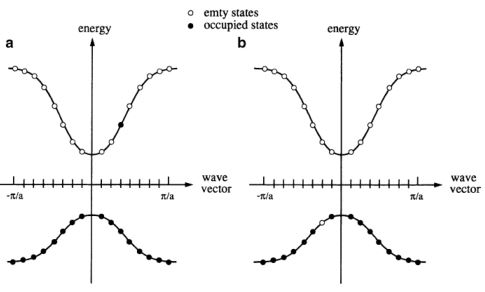
\includegraphics[clip,width=9cm]{8_6.JPG}
  \caption{$N\pm1$粒子問題を表している伝導帯における1つの電子(a)と価電子帯における1つの正孔(b).(黒点:占有状態、白点:空の状態)}
  \label{8.6}
\end{figure}
\fi

\setcounter{section}{12}%次のsectionはn+1から
\setcounter{subsection}{0}
\setcounter{figure}{0}
\newpage
\section{バルク半導体中の固有励起子の光学特性}
フォノンやプラズモン、マグノンの光学特性を扱う際に、これ以降の章から、半導体光学の本質、つまり励起子の光学特性にたどり着く。

フォノンは、半導体の特性や、赤外の絶縁体について述べるのに必要で、プラズモンは、赤外から可視域に近い紫外までの金属や半導体の光学特性を決定し、もしあるならば、それらはフォノンとともにIRスペクトルに寄与する。励起子は、一方で、continuum stats(連続体統計?)やバンド間遷移と共に、バンドギャップ周辺およびそれ以上、すなわち、半導体の場合は紫外や赤外の近くを含む可視域、絶縁体の場合は(真空)紫外線の光学特性について決定する。アルカリハロゲン化物のような無機絶縁体やアントラセンのような有機半導体は特定の光学特性を有しているが、側面の多くは、これ以降、それらにも適用できるような、半導体中の励起子を提示する。

9章の冒頭ですでに、励起子の研究の歴史の情報のいくつかを与えている。例えば、[44M1,52H1,53U1,57E1,57M1,58D1,59M1,60H1,62H1,62P1,63H1,66V1]などの最近の参照のいくつかをここで再び集め、半導体の分光法のいくつかのさらなる参照を[40K1,54K1]で与え、最近の審査[63P1,81R1]を引用する。

\subsection{強い振動子強度での励起子}
この章では、最も強い振動子強度において双極子許容励起子を示すような、双極子許容の、バンド間遷移から始まるバルク半導体中の固有励起子の線形光学特性に集中する。縦横分裂の値$\Delta_{\mathrm{LT}}$の範囲は0.1\,meVから10\,meVである。

注意されるべきこととして、しかし、半導体のこのグループのすべての励起子が強い振動子強度を持つわけではなく、また、双極子禁制バンド間遷移半導体中のいくつかの励起子は、低い振動子強度ではあるが、双極子許容である。

\subsubsection{励起子-光子結合}
双極子許容直接バンド間遷移半導体では、励起子が発生した時、放射場と強く結合する。結果として多くの光学特性が、強結合かポラリトンの図で定量的に理解される。それゆえ、古典的教義「反復は勉学の母である」に気を付けながら、1つ以上の特別な場合の放射場との強い、あるいは弱い結合、を解明するのにこの機会を用いる。

2.1-2.6章で、電磁放射場について、2.5章で量子としての光子について紹介した。9-11章では、様々な初等の励起子の特性について説明した。2つの相互作用は摂動理論で扱われる。これは弱い結合近似と呼ばれる。1光子吸収係数$\alpha(\omega)$はこのとき、(13.1a)のように双極子行列要素の平方の共鳴比例であり、すなわち、始状態と終状態の1次摂動理論から求まる。

%13.1a

屈折率は、$\alpha(\omega)$のKramers-Kronig変形か、共鳴から離れて、(13.1b)のよる2次摂動理論か、のどちらかの近似のこのレベルで得られる。

%13.1b

光子$\hbar\omega$は、事実上、$\Delta t$秒後に(13.2)のように制限された運動量の保存の下、励起された中間状態$|z>$を創り、

%13.2

入射されら光子と同一の光子を再び放出し、電子系は初期状態$|i>$に戻る。エネルギーが仮想励起状態に「保存」されている時間$\Delta t$の間

\end{document}
